\documentclass[12pt]{article}
\usepackage[a4paper, margin=1in]{geometry}
\usepackage{graphicx}
\usepackage{hyperref}

\usepackage{natbib}
\bibliographystyle{ieeetr}
\setcitestyle{super,open={[},close={]}}

\title{Title}
\author{Marco Coppola,\\
Valerio Pio De Nicola,\\
Davide De Rosa \\ \\
University of Bologna}
\date{}

\begin{document}

\maketitle

\section{Introduction}
per la fine

\section{InstructLab}
\subsection{Introduction to LAB}
Large language models (LLMs) have achieved success in NLP tasks due to the transformer architecture. LLM training consists of two main phases: \textbf{pre-training} (which is computationally expensive and involves predicting the next token using massive datasets) and \textbf{alignment tuning} (which refines model behavior through instruction and preference tuning).\vspace{14pt}\\
Pre-training dominates the resource cost, while alignment tuning, including instruction tuning (training on task-specific instructions) and preference tuning (using human feedback methods like RLHF), requires significantly fewer data and compute resources.\\
Despite this, alignment tuning is crucial for optimizing LLMs for real-world use.\vspace{14pt}\\
To address challenges in scaling alignment tuning, the \textbf{LAB} (\textbf{Large-scale Alignment for chatBots}\cite{sudalairaj2024lablargescalealignmentchatbots}) \textbf{method} has been recently created. LAB includes:
\begin{enumerate}
    \item \textbf{Synthetic data generation} guided by taxonomy and quality assurance, avoiding reliance on proprietary LLMs or extensive human curation.  
    \item \textbf{A novel multi-phase training framework} that integrates new knowledge without causing catastrophic forgetting.
\end{enumerate}
LAB-trained models achieve competitive performance compared to those using human-annotated or GPT-4-generated data, demonstrating its effectiveness for improving LLM instruction-following capabilities.\vspace{14pt}\\
Recent advancements in instruction tuning for large language models (LLMs) have primarily relied on two key methodologies: \textbf{human-annotated datasets} and \textbf{synthetic data generation}. Traditional approaches, such as those pioneered by OpenAI and later adopted by the creators of LLaMA 2, emphasize the collection of high-quality human-generated data. This process involves extensive human annotation efforts, requiring rigorous selection and training of annotators to ensure consistency and quality.\vspace{14pt}\\
While effective in aligning models with human preferences, these methods are resource-intensive, costly, and often slow, limiting the ability to rapidly explore new instruction types and model capabilities.
To address these limitations, synthetic data generation has emerged as an alternative, leveraging LLMs to produce instruction-tuning datasets.\vspace{14pt}\\
Early efforts, such as Self-Instruct, introduced a bootstrapping approach that expands a small set of human-written seed instructions into a large dataset using an LLM’s own generation capabilities. Subsequent refinements sought to enhance data diversity and instruction complexity through iterative and principled augmentation techniques.\\
Other works have further extended this approach by focusing on task diversity and progressive training frameworks, incorporating richer reasoning signals to improve model performance incrementally.\vspace{14pt}\\
More recently, semi-automated techniques, such as GLAN, have introduced a structured approach to synthetic data generation by leveraging human-curated taxonomies.\\
However, such methods remain constrained by the limitations of the teacher model used for data generation, particularly when relying on proprietary models like GPT-4, which impose restrictions on the commercial usability of the generated data.\vspace{14pt}\\
In contrast, open-source approaches, such as LAB, attempt to mitigate these concerns by employing models like Mixtral, allowing for greater flexibility in data generation and application.\vspace{14pt}\\
The ongoing evolution of instruction tuning methods highlights the trade-offs between human-annotated and synthetic data-driven approaches.\\
While human-generated data ensures high-quality alignment, it is costly and inflexible.\\
Conversely, synthetic data techniques offer scalability and efficiency but introduce challenges related to data diversity, quality control, and legal constraints surrounding proprietary models.\\
Future research will likely focus on hybrid approaches that balance these trade-offs, incorporating the strengths of both methodologies to enhance the instruction-tuning process.

\subsection{How does LAB work}
LAB is a structured framework designed to enhance instruction tuning through a combination of systematic data curation and multi-phased training. It consists of two key components:
\begin{itemize}
    \item \textbf{Taxonomy-Guided Synthetic Data Generator}: this component facilitates data curation by organizing instructions into a structured taxonomy. It also plays a crucial role in guiding the synthetic data generation process, ensuring both high diversity and quality in the instruction-tuning dataset. By leveraging a well-defined taxonomy, LAB aims to improve the comprehensiveness and relevance of the generated data.
    \item \textbf{Multi-Phased Instruction-Tuning with Replay Buffers}: to maintain training stability and mitigate issues such as catastrophic forgetting, LAB employs a multi-stage tuning approach. The use of replay buffers allows the model to retain previously learned information while adapting to new instructions, thereby improving overall alignment performance.
\end{itemize}
Together, these components form an end-to-end pipeline for aligning a pre-trained LLM, as illustrated in Figure~\ref{fig:ilab}. This approach balances synthetic data diversity with training stability, making it a scalable and effective method for large-scale instruction tuning.\\
\begin{figure}
    \centering
    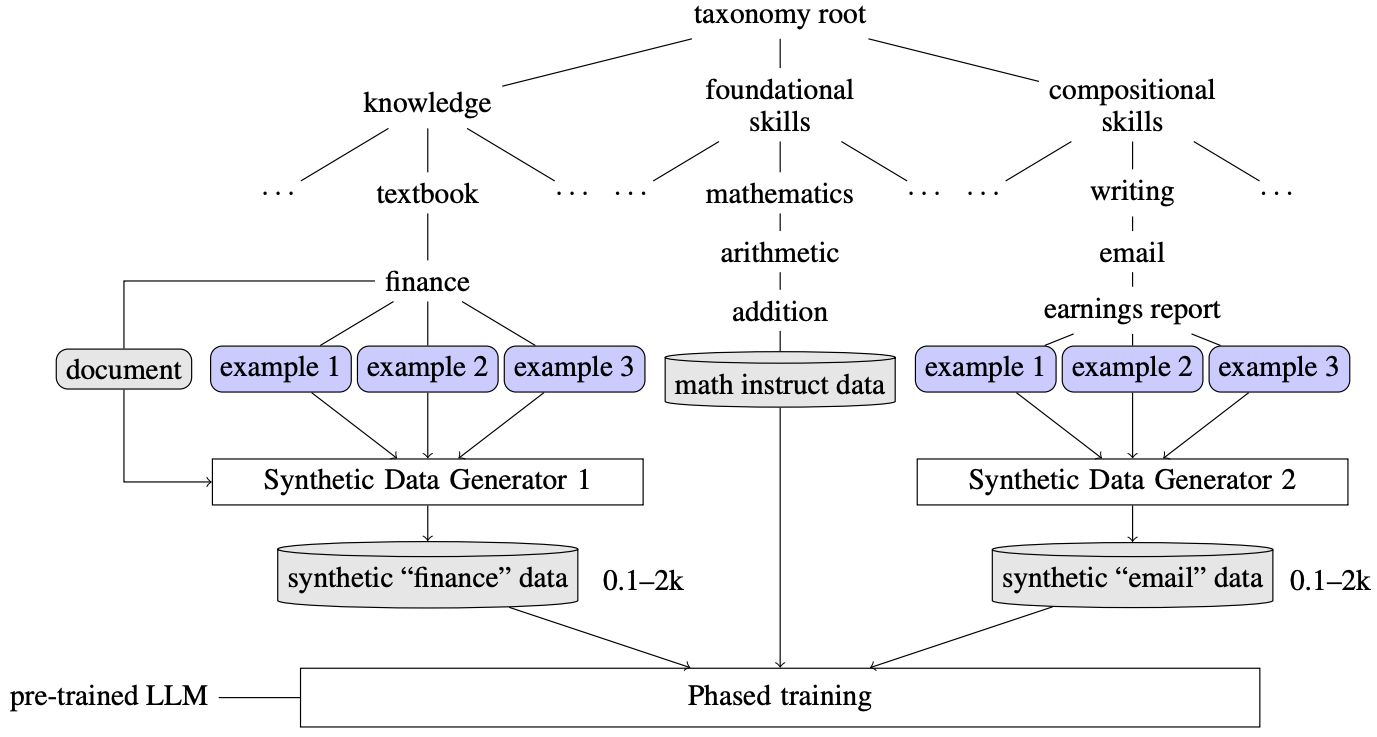
\includegraphics[width=1\textwidth]{img/figure1.png}
    \caption{\textit{Overview of the LAB alignment method. Starting from the taxonomy root, data are curated in each top-level groups and examples in the leaf nodes are used by the synthetic data generators to generate orders of magnitude data for the phased-training step for instruct-tuning.}}
    \label{fig:ilab}
\end{figure}

\subsubsection{Taxonmy}
LAB's taxonomy serves as a structured framework for organizing instruction-tuning data, enabling systematic curation and enhancement of training datasets. It hierarchically classifies data samples into three main branches: \textbf{knowledge}, \textbf{foundational skills}, and \textbf{compositional skills}. Each of these branches is further subdivided into more granular levels, with specific tasks defined at the leaf nodes. These leaf nodes are exemplified by manually written instruction-response pairs, ensuring clarity in task representation.\vspace{14pt}\\
This hierarchical organization provides several advantages.\vspace{14pt}\\
First, it allows model designers and data curators to identify gaps in the model’s capabilities by pinpointing missing or underrepresented tasks.\vspace{14pt}\\
Second, it facilitates the incremental expansion of training data, as new tasks can be seamlessly integrated by adding a leaf node under the appropriate branch, accompanied by 1–3 examples.\vspace{14pt}\\
This structured approach ensures that instruction tuning remains both comprehensive and adaptable, improving the overall alignment and robustness of the trained LLM.\vspace{14pt}\\
\textbf{Knowledge}\\
The \textit{Knowledge} branch categorizes domain-specific documents like textbooks and research papers. It ensures ethical synthetic data generation by selecting only licensed content.\vspace{14pt}\\ 
\textbf{Foundational Skills}\\
The \textit{Foundational Skills} branch includes core abilities like math, coding, and reasoning. Public datasets support structured learning for effective generalization.\vspace{14pt}\\
\textbf{Compositional Skills}\\
The \textit{Compositional Skills} branch integrates knowledge and foundational skills for complex tasks. It enables models to synthesize information for coherent, multi-step responses.

\subsubsection{Taxonomy-Driven Synthetic Data Generator}\label{tax-sdg}
LAB enhances \textbf{synthetic data generation} (\textbf{SDG}) by leveraging a \textit{taxonomy-driven approach} rather than relying on traditional random sampling methods.\\
While manually curated data samples embedded in the taxonomy’s leaf nodes can be used for direct instruction tuning, prior research suggests that a large volume of high-quality instruction data is necessary for improving instruction-following capabilities in LLMs.\vspace{14pt}\\
Existing SDG methods attempt to scale synthetic data generation using teacher models, but they suffer from mode collapse — over-representing the dominant patterns of the teacher model while neglecting diverse or less common instruction types.\vspace{14pt}\\
This limitation arises from random selection of seed examples, which results in prompts that reflect an "average" of the dataset rather than task-specific examples. Consequently, the teacher model generates synthetic data that predominantly aligns with its dominant distribution while ignoring the long-tail of diverse or nuanced tasks. To overcome this, LAB replaces random selection with taxonomy-driven sampling, ensuring that data generation is targeted at the level of individual leaf nodes. This approach guarantees balanced representation across different instruction types, preventing bias toward a subset of commonly occurring prompts.\vspace{14pt}\\
LAB introduces two new SDG methods based on this taxonomy-guided framework:
\begin{enumerate}
    \item \textbf{Skills Generation}: this method uses the task examples stored in the leaf nodes to generate a larger dataset using the open-source \textbf{Mixtral-7x8B model}. By focusing on specific skill categories, LAB ensures better diversity and task-specific representation in the synthetic data.  
    \item \textbf{Knowledge Generation}: unlike prior approaches that rely on a teacher model’s internal knowledge, LAB’s knowledge generation method still employs \textbf{Mixtral-7x8B}, but without depending on pre-existing knowledge stored in the model. This approach mitigates biases introduced by the teacher model’s knowledge limitations while maintaining control over the source material used for synthetic data creation.  
\end{enumerate}
By structuring data generation around the taxonomy, \textbf{LAB improves both the diversity and quality} of synthetic instruction-tuning datasets, addressing key weaknesses in traditional SDG pipelines.\vspace{14pt}\\
\textbf{Skill Generation}\\
Skills-SDG follows a structured, multi-stage approach to generate diverse, high-quality instructional data using Mixtral-7x8B. Four specialized prompts guide the teacher model in different roles:  
\begin{enumerate}  
    \item \textbf{Instruction Generation}: the model generates diverse, well-structured instructions by systematically exploring taxonomy nodes.  
    \item \textbf{Evaluating Instructions}: instructions are filtered for relevance, safety, and feasibility, ensuring only high-quality queries proceed.  
    \item \textbf{Generating Responses}: responses are tailored per domain, ensuring creativity for writing tasks and precision for STEM subjects.  
    \item \textbf{Evaluating Instruction-Response Pairs}: a rating system filters out inaccurate or off-topic samples, ensuring high-quality data.  
\end{enumerate}
\textbf{Knowledge Generation}\\
Knowledge-SDG addresses SDG limitations by grounding data generation in external sources like manuals and books, reducing hallucinations. Unlike conventional SDG, this method ensures factual accuracy by integrating structured examples with external knowledge. The teacher model evaluates content to maintain reliability, making this approach particularly valuable for specialized domains.  

\subsection{What's under the hood}
Fine-tuning large language models (LLMs) on consumer hardware presents significant challenges due to high computational and memory demands. To address these challenges, we leverage the ILAB framework, which integrates several optimization techniques: Synthetic Data Generation (SDG), Model Quantization, Low-Rank Adaptation (LoRA\cite{hu2021loralowrankadaptationlarge}), and Quantized LoRA (QLoRA\cite{dettmers2023qloraefficientfinetuningquantized}). These methods work together to enable efficient training and adaptation of LLMs on consumer-grade GPUs.

\subsubsection{Synthetic Data Generation (SDG)}
SDG enhances the training process by generating high-quality synthetic data, reducing the dependence on large real-world datasets. This not only helps in domain adaptation but also mitigates data scarcity issues, improving model generalization.

\subsubsection{Model Quantization}
Model quantization reduces the precision of model parameters (e.g., from 16-bit floating point to 8-bit integers), significantly lowering memory requirements and computational costs. This enables larger models to fit within the limited VRAM of consumer GPUs while maintaining near-original performance.

\subsubsection{Low-Rank Adaptation (LoRA)}
LoRA fine-tunes LLMs efficiently by introducing low-rank matrices into selected layers instead of updating all model parameters. This dramatically reduces the number of trainable parameters, making fine-tuning feasible on constrained hardware.

\subsubsection{Quantized LoRA (QLoRA)}
QLoRA combines the benefits of quantization and LoRA by applying quantization techniques to the base model while training LoRA adapters on top. This further reduces memory consumption, allowing large-scale models to be fine-tuned even on GPUs with limited VRAM.

\subsubsection{How These Techniques Work Together}
By combining these methods, ILAB creates a highly efficient fine-tuning pipeline.
\begin{itemize}
    \item SDG provides a diverse training dataset, enhancing model robustness
    \item Model quantization compresses the base model, reducing memory footprint
    \item LoRA then enables efficient fine-tuning without modifying the entire model, and
    \item QLoRA further optimizes this by applying quantization to the base model while keeping adapter layers in higher precision.
\end{itemize}
This synergy allows consumer hardware, such as NVIDIA RTX-series GPUs, to fine-tune large-scale LLMs that would otherwise require enterprise-level infrastructure.

\subsection{Output Model: GGUF Format with Llama CPP Runner}\label{gguf}
After fine-tuning the large language model (LLM) using the ILAB framework, the resulting model is saved in the GGUF (GPT-Generated Unified Format) format.\\
GGUF is a highly efficient format designed for easy deployment and fast inference, ensuring that the model can be loaded and run with minimal overhead on a variety of hardware configurations. This format is particularly well-suited for use with the Llama CPP runner, which is a lightweight inference engine designed for high-performance model execution.\\
One of the key advantages of the GGUF format, when paired with the Llama CPP runner, is its seamless compatibility with Apple's hardware ecosystem. Apple Silicon (M1, M2, and future generations) is considered a first-class citizen in this setup, benefiting from optimized performance through the use of several native technologies, including ARM NEON, Accelerate, and Metal frameworks.\\
This optimized execution on Apple Silicon enables efficient use of consumer hardware, making it possible to run the fine-tuned model with minimal latency and power consumption, even on relatively modest devices.\vspace{14pt}\\
LAB enables practical fine-tuning of LLMs on consumer hardware by leveraging SDG, model quantization, LoRA, and QLoRA. These techniques collectively reduce memory requirements, computational overhead, and data dependency, making LLM fine-tuning and inference accessible beyond high-performance data centers.

\section{Our Work}
Our main goal was to fine-tune a Large Language Model (LLM) to help us write Jolie\footnote{https://www.jolie-lang.org/} code on consumer hardware (our PCs). We started by looking for tools that would help us achieve this task. We found IBM's InstructLAB\footnote{https://instructlab.ai/}, which is still in the early stages of development.\vspace{14pt}\\
After an initial phase of studying the tool's documentation, we began by installing the tool.

\subsection{Installing ILAB}
ILAB is essentially a Python package, so it can be installed using pip in your virtual environment with the following command:
\begin{center}
    \texttt{pip install instructlab}
\end{center}
During the installation process, you need to set various parameters to enable GPU acceleration and other features. You can set up all the necessary parameters in your environment by running the following command:
\begin{center}
    \texttt{ilab config init}
\end{center}
Our main machine for this project was an \textit{M1 Pro MacBook Pro 14}, with 16GB of RAM. We also used our department's HPC for various tests before settling on the MacBook.\vspace{14pt}\\
After installing and setting everything up, we created the taxonomy.

\subsection{Creating the Taxonomy}
ILAB's taxonomy consists of different "leaves" called QnA (Questions and Answers) in YAML format. Each leaf covers a single topic.\\
These files are quite simple. An example of our Introduction to Jolie QnA is shown below:
\begin{center}
    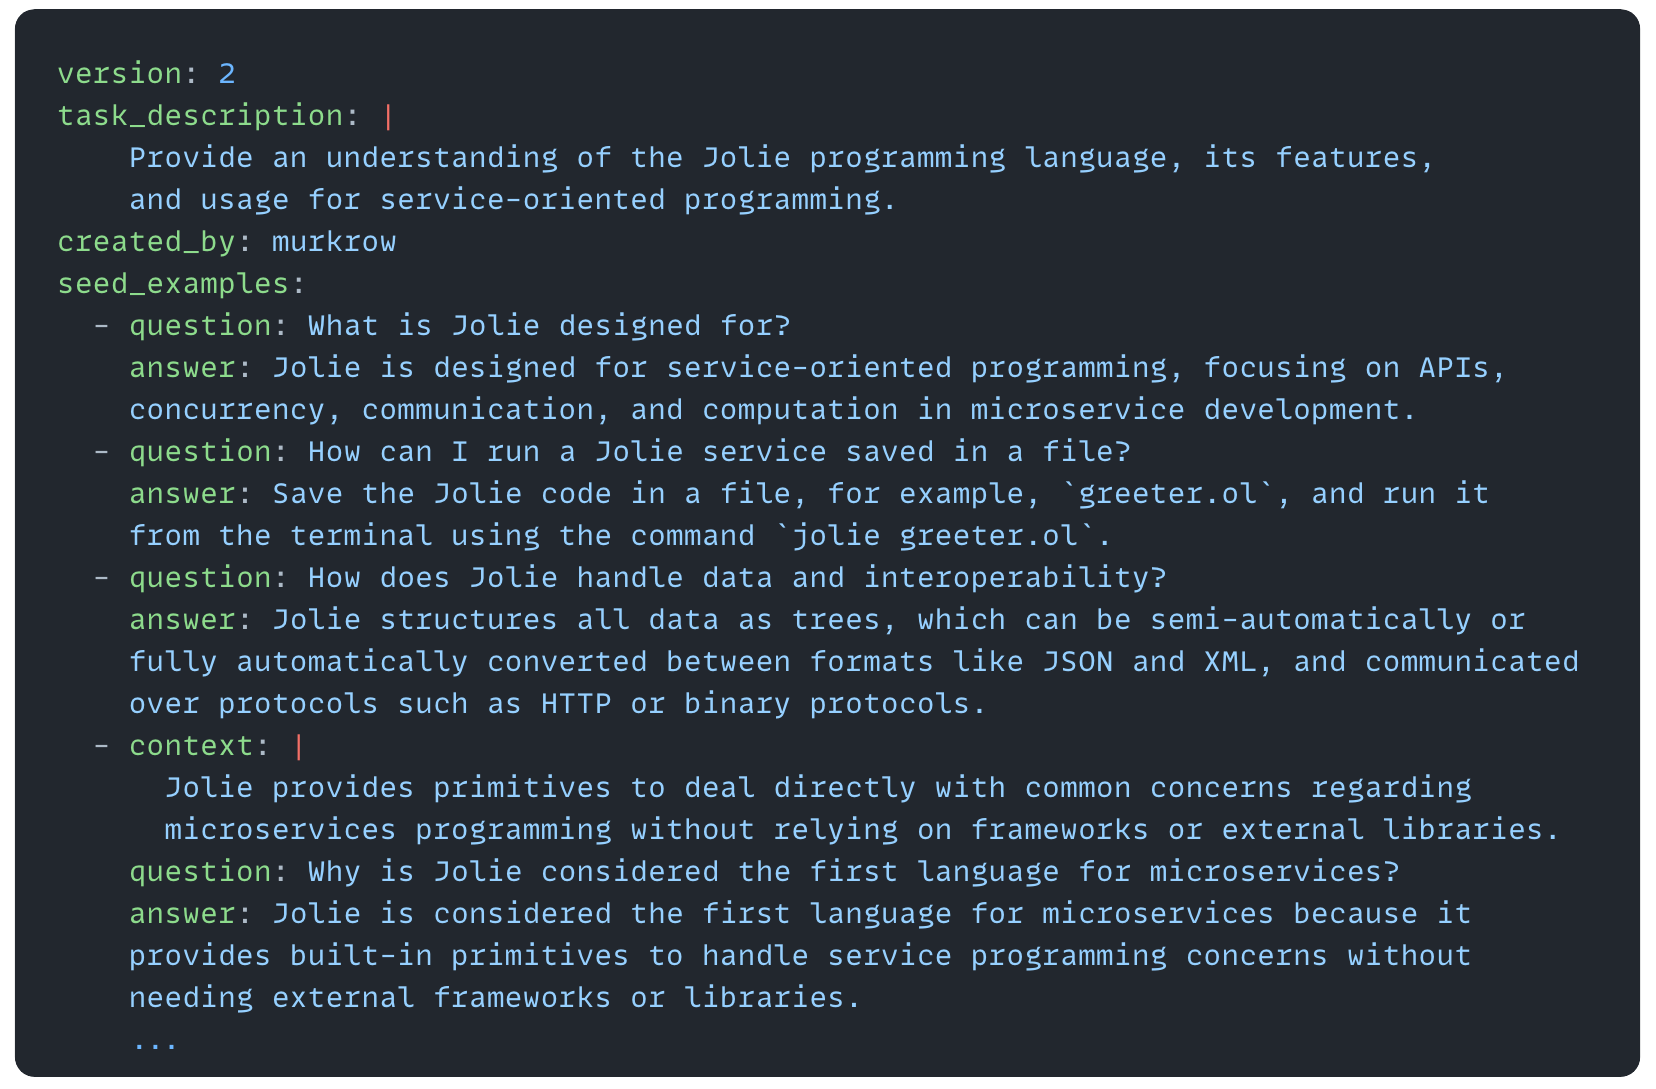
\includegraphics[width=0.9\textwidth]{img/qna.png}
\end{center}
We used Jolie's documentation\footnote{https://docs.jolie-lang.org/v1.13.x-git/introduction/index.html} to create QnAs for every part of the language's documentation.\\
ILAB provides a tool to validate the different QnAs using the following command:
\begin{center}
    \texttt{ilab taxonomy diff}
\end{center}
Once we created all the QnAs for the documentation, we used ILAB to convert the taxonomy into datasets.

\subsection{Dataset Generation}
This is where the SDG parts come into play. ILAB uses an instructor LLM to generate datasets by expanding the taxonomy into larger text files, as discussed in section [\ref{tax-sdg}]. In our case, we used \textit{Mixtral-8x7B} as the teacher model — the default teacher model for ILAB — which can be downloaded using the following command:
\begin{center}
    \texttt{ilab model download --hf-token=*}
\end{center}
Generating datasets on our Apple machine was, to say the least, \textit{buggy}. We chose to use the HPC to run this task, which took almost 60 hours on an RTX 2080. If the tool had worked properly, we could have run it on our own machine as well.\\
To generate the datasets, we used the following command:
\begin{center}
    \texttt{ilab data generate --pipeline simple}
\end{center}
The "simple" flag for the pipeline is used for training on Apple machines.\vspace{14pt}\\
We can now move on to the training phase.

\subsection{Training the Base Model}
Once the datasets were ready, we used the following command to start training the base model:
\begin{center}
    \texttt{ilab model train --pipeline simple --local --num-epochs * --iters * --optimize-memory}
\end{center}
We ran this command multiple times to create several models with different iteration counts. We chose not to change the number of epochs — always set to 1 — because the process was somewhat buggy. For our case study, we settled on 100, 250, 500, and 1000 iterations.\vspace{14pt}\\
Once all the models were created and ready to use, the final step was to convert them to \textit{.gguf} format to quantize them.

\subsection{Model Quantization}
This step was necessary in order to \textit{serve} the models, as there is currently no way to run safetensors files on Apple machines. The only available runner is \textbf{LLama.cpp}, which requires a .gguf file [\ref{gguf}]. For each conversion, we used the following command:
\begin{center}
    \texttt{ilab model convert --model-name jolieLLM}
\end{center}
The last, and most interesting, step was to chat with the newly created models.

\subsection{Serving and Chatting with the Models}
ILAB allows you to chat with the model by serving it. You can do so using the following command:
\begin{center}
    \texttt{ilab model serve --model-path ./jolieLLM.gguf}
\end{center}
Once the model is being served, you can chat with it using the following command:
\begin{center}
    \texttt{ilab model chat}
\end{center}

\section{Our case study}
ciao

\section{Trying to visualize the attention mechanism}

\pagebreak

\bibliography{ref.bib}
\end{document}